%%%%%%%%%%%%%%%%%%%%%%%%%%%%%%%%%%%%%%%%%%%%%%%%%%%%%%%%%%%%%%%%%%%%%%%%%%%%%%%%
%2345678901234567890123456789012345678901234567890123456789012345678901234567890
%        1         2         3         4         5         6         7         8

\documentclass[letterpaper, 10 pt, conference]{ieeeconf}  % Comment this line out if you need a4paper

%\documentclass[a4paper, 10pt, conference]{ieeeconf}      % Use this line for a4 paper

\IEEEoverridecommandlockouts                              % This command is only needed if
                                                          % you want to use the \thanks command

\overrideIEEEmargins                                      % Needed to meet printer requirements.

%In case you encounter the following error:
%Error 1010 The PDF file may be corrupt (unable to open PDF file) OR
%Error 1000 An error occurred while parsing a contents stream. Unable to analyze the PDF file.
%This is a known problem with pdfLaTeX conversion filter. The file cannot be opened with acrobat reader
%Please use one of the alternatives below to circumvent this error by uncommenting one or the other
% \pdfobjcompresslevel=0
% \pdfminorversion=4

% See the \addtolength command later in the file to balance the column lengths
% on the last page of the document

% The following packages can be found on http:\\www.ctan.org
\usepackage{graphics} % for pdf, bitmapped graphics files
\usepackage{graphicx}
%\usepackage{epsfig} % for postscript graphics files
%\usepackage{mathptmx} % assumes new font selection scheme installed
%\usepackage{times} % assumes new font selection scheme installed
\usepackage{amsmath} % assumes amsmath package installed
\usepackage{amssymb}  % assumes amsmath package installed
\usepackage{subfig}
\usepackage[hidelinks]{hyperref}
\usepackage{float}
\usepackage{multirow}

\makeatletter
\g@addto@macro{\UrlBreaks}{%
\do\/\do\a\do\b\do\c\do\d\do\e\do\f%
\do\g\do\h\do\i\do\j\do\k\do\l\do\m%
\do\n\do\o\do\p\do\q\do\r\do\s\do\t%
\do\u\do\v\do\w\do\x\do\y\do\z%
\do\A\do\B\do\C\do\D\do\E\do\F\do\G%
\do\H\do\I\do\J\do\K\do\L\do\M\do\N%
\do\O\do\P\do\Q\do\R\do\S\do\T\do\U%
\do\V\do\W\do\X\do\Y\do\Z}
\makeatother

\newcommand\norm[1]{\left\lVert#1\right\rVert}

\title{\LARGE \bf
Visual Servoing and Reinforcement Learning for Robotic Control
}


\author{Steven Tang$^{1}$ and Martin Jagersand$^{1}$% <-this % stops a space
\thanks{*We acknowledge the support of the Natural Sciences and Engineering Research
Council of Canada (NSERC).}% <-this % stops a space
\thanks{$^{1}$Department of Computing Science, University of Alberta, Edmonton
    AB., Canada, T6G 2E8. {\tt\small \{stang5, mj7\}@ualberta.ca}}%
}


\begin{document}



\maketitle
\thispagestyle{empty}
\pagestyle{empty}


%%%%%%%%%%%%%%%%%%%%%%%%%%%%%%%%%%%%%%%%%%%%%%%%%%%%%%%%%%%%%%%%%%%%%%%%%%%%%%%%
\begin{abstract}
    This paper explores visual servoing and reinforcement learning for robotic
    control. In a simulated reaching task, we investigate the performance and
    sample efficiency of uncalibrated visual servoing and reinforcement
    learning. We analyze different reward functions and representations for the
    policy. We experiment with methods that combine visual servoing and
    reinforcement learning. Our experiments compare and contrast these
    approaches to provide insight into their strengths and weaknesses
    in hand eye coordination tasks.
\end{abstract}


%%%%%%%%%%%%%%%%%%%%%%%%%%%%%%%%%%%%%%%%%%%%%%%%%%%%%%%%%%%%%%%%%%%%%%%%%%%%%%%%
\section{INTRODUCTION}

Humans use hand-eye coordination to perform many day to day tasks including
reaching for objects. In robotics, there has been significant research in this
field. Hand-eye coordination tasks decompose into perception
which maps high dimensional image space to a lower visual feature space,
control based on camera-robot geometry, and a method for task specification.

Visual servoing is one method used to perform these tasks without explicit
modeling of the robot visuomotor function and the use of absolute world
coordinate systems. Typically, in visual servoing, the robot uses visual video
tracking to perform perception and online Jacobian learning is used to learn how
to control the robot, tasks are specified by visual selection.
\cite{Jagersand1995} Generally, visuals servoing methods have low sample
complexity, as the Jacobian can be initialized with a central difference method.
However, the Jacobian is a locally linear approximation of the visuomotor
function, so it is very accurate locally, but not necessarily convergent
globally.

In contrast, deep reinforcement learning (RL) has also been used to learn hand-eye
coordination tasks in robotics. \cite{Levine15} Neural networks are used to approximate
an end to end policy that maps visual observations to actions. Usually, convolutional
neural networks are used to extract features from the visual observations, while fully
connected neural networks are used to map the features to actions. Reinforcement
learning methods require more samples from the environment to learn compared to visual
servoing methods, but they are more general in that reward is sufficient for task
specification and can learn a global motor policy.

Visual servoing and reinforcement learning are two quite different methods that can be
used to perform hand-eye coordination tasks. In particular, we study how the different
methods of visual servoing and reinforcement learning in the context of learning
camera-robot geometry for robotic control. We use tracked points for perception and
visual selection for task specification for both methods. We report quantitative
performance data comparing the different methods in terms of sample complexity and
overall performance in a simulated reaching task. Furthermore, we study how the two
methods can be combined to get the best of both methods.

In Section \ref{Background}, we provide background information on visual
servoing and reinforcement learning. In Section \ref{Related Works}, we discuss
similar works in the literature. In Section \ref{Methodology}, we describe
the methods we explore in our experiments. In Section \ref{Experiments}, we
describe our experimental setup and share our results. In Section
\ref{Conclusion}, we conclude our work and discuss future work.

\section{BACKGROUND} \label{Background}

\subsection{Visual Servoing}

Visual servoing is a robot control technique using vision. There are
two main types of visual servoing. In calibrated visual servoing, the camera
calibration parameters are known. \cite{Chaumette2006} On the other hand, uncalibrated visual
servoing relies on only on image features to control the robot, reducing the
amount of calibration effort and is more general
and independent of the specific experimental setup.
Previous experiments have shown visual servoing to be an effective method for
\cite{Jagersand1997} hand-eye coordination tasks. We focus on uncalibrated
visual servoing with two fixed cameras.

Let $\mathbf{q} \in \mathbb{R}^d$ be
the $d$-DOF robot's joint angles, $(u_{e_1}, v_{e_1}), (u_{e_2}, v_{e_2})$ be the image features of the end
effector from the first and second cameras, and $(u_{g_1}, v_{g_1}), (u_{g_2}, v_{g_2})$ be the image
features of the goal from the first and second cameras.

The point to point
error vector $\mathbf{f}(\mathbf{q})$ is a non-linear function of the joint angles
$\mathbf{q}$. In uncalibrated visual servoing, we seek to minimize this error.
\begin{equation}
    \mathbf{f}(\mathbf{q}) = \begin{bmatrix}
        u_{g_1} - u_{e_1} \cr
        v_{g_1} - v_{e_1} \cr
        u_{g_2} - u_{e_2} \cr
        v_{g_2} - v_{e_2}
    \end{bmatrix}
\end{equation}

Given the Jacobian $\mathbf{J}$, we can use Newton's method to solve
for the $\Delta \mathbf{q}$ that minimizes a linear approximation of the error
function.

\begin{equation}
    \mathbf{J}_{\mathbf{f}}(\mathbf{q}) \Delta \mathbf{q} = -\mathbf{f}(\mathbf{q})
\end{equation}

The update to the joint angles $\Delta \mathbf{q}$ is given by
\begin{equation}
    \Delta \mathbf{q} = -\mathbf{J}_{\mathbf{f}}(\mathbf{q})^{+} \mathbf{f}(\mathbf{q})
\end{equation}

Where $\mathbf{A}^{+}$ is the Moore-Penrose pseudoinverse of $\mathbf{A}$. The
robot controller is then given the update to the joint angles $\Delta \mathbf{q}$,
and the joint angles are updated using the following equation.

\begin{equation}
    \mathbf{q}_{t+1} = \mathbf{q}_t + \Delta \mathbf{q}_t
\end{equation}

The Jacobian $\mathbf{J}_{\mathbf{f}}(\mathbf{q})$ is initialized with the
central difference approximation. We can estimate each column independently,
perturbing one joint, keeping the other joints fixed.

\begin{equation}
    \mathbf{J}_{\mathbf{f}}(\mathbf{q})_i = \frac{\mathbf{f}(\mathbf{q} + \epsilon \mathbf{e}_i) - \mathbf{f}(\mathbf{q} - \epsilon \mathbf{e}_i)}{2 \epsilon}
\end{equation}

Where $\mathbf{J}_{\mathbf{f}}(\mathbf{q})_i$ is $i$-th column of the Jacobian,
the $\mathbf{e}_i$ is the $i$-th standard unit vector, using a small
perturbation $\epsilon$, in our case, $0.1$ radians.

The Jacobian $\mathbf{J}_{\mathbf{f}}(\mathbf{q})$ approximation can be updated online
using Broyden's method.
\begin{equation}
    \mathbf{J}_{\mathbf{f}}(\mathbf{q})_{t+1} = \mathbf{J}_{\mathbf{f}}(\mathbf{q})_t + \frac{\mathbf{f}(\mathbf{q})_t - \mathbf{J}_{\mathbf{f}}(\mathbf{q})_t \Delta \mathbf{q}_t}{\Delta \mathbf{q}_t^\top \Delta \mathbf{q}_t} \Delta \mathbf{q}_t^\top
\end{equation}

\subsection{Reinforcement Learning}

On the other hand, reinforcement learning learns from interaction with
the environment. RL acts in a Markov Decision Process (MDP) defined by the tuple
$(\mathcal{S}, \mathcal{A}, \mathcal{P}, \mathcal{R}, \gamma)$ where $\mathcal{S}$ is
the state space, $\mathcal{A}$ is the action space, $\mathcal{P}$ is the transition
probability function, $\mathcal{R}$ is the reward function, and $\gamma \in [0, 1]$ is the discount
factor. The environment takes in an action and returns the next state and reward
according to the transition probability function and reward function respectively.

The objective of the robot agent is to learn a policy $\pi(\mathbf{s}_t) =
\mathbf{a}_t$ that maps states from the environment to actions which maximizes
the expected return $R = \mathbb{E}[\sum_{t=0}^T \gamma^t r_t]$ where $r_t$ is
the reward at time $t$, and $T$ is the time horizon. Often, deep neural networks are used to represent the policy.
The policy is learned using gradient descent methods to maximize the expected
return.

The reaching task can be viewed as an episodic MDP. The episode ends when the end
effector is within a threshold distance of the target position. The state vector
consists of the joint angles concatenated with the image features of the end effector
and goal positions.

\begin{equation}
    \mathbf{s} = \begin{bmatrix}q_1, \ldots, q_d, u_{e_1}, v_{e_1}, u_{e_2}, v_{e_2}, u_{g_1}, v_{g_1}, u_{g_2}, v_{g_2}\end{bmatrix}^\top
\end{equation}

The action vector is the update to the joint angles, $\mathbf{a} = \Delta q$.

\section{RELATED WORKS} \label{Related Works} In \emph{Model-based and model-free
reinforcement learning for visual servoing} Farahmand et al. introduces
model-based and model-free RL methods for visual servoing. \cite{Farahmand2009}
They compare the performance of model-based RL, model-free RL, and uncalibrated
visual servoing using only the first 3 DOF of the robot with discrete actions.
In our work, we compare the performance of uncalibrated visual servoing and
reinforcement learning using 3, 4, and 7 DOF robots with continuous actions.

In \emph{End-to-End Training of Deep Visuomotor Policies}, Levine et al. discuss
end-to-end training of deep visuomotor policies, using guided policy search,
which combines supervised learning with a trajectory-centric RL algorithm that
provides supervision on the policy. They evaluated their technique on a range of
real-world manipulation tasks.
\cite{Levine15}

In \emph{Asynchronous Reinforcement Learning for Real-Time Control of Physical
Robots}, Yuan and Mahmood demonstrate a system that learns to reach visual
targets from pixels within 2 hours of experience using a real 5 DOF robot.
\cite{Yuan2022} The paper's focus is on evaluating sequential and asynchronous
learning, but serves as a good example of developing practical RL systems for
real world visual robotic control.


\section{METHODOLOGY} \label{Methodology}

\subsection{Representation}

In the uncalibrated visual servoing problem, we consider
the representation of the visuomotor function to be the Jacobian which
is learned using Broyden's method. In reinforcement learning, we consider
neural networks and a Neural Jacobian approach to represent the visuomotor
function.

\subsubsection{Neural Networks}

Commonly used in reinforcement learning, neural networks are used to represent
the policy.

In our case, we use fully
connected neural networks parameterized by $\theta$ to approximate the end to
end policy. We compare the performance of different neural network
architectures, including the number of layers and the number of neurons per
layer. We use the rectified linear unit, $\text{ReLU}$,
activation function for hidden layers, and $\tanh$ for the output layer. We use
the Adam optimizer with a learning rate of $0.001$.

For example, a 2-layer neural network with $l$ neurons per layer is given by
\begin{equation}
    \pi_\theta(\mathbf{s}) = \tanh(\mathbf{W}_2 \text{ReLU}(\mathbf{W}_1 \mathbf{s} + \mathbf{b}_1) + \mathbf{b}_2)
\end{equation}
Where $\mathbf{W}_2 \in \mathbb{R}^{d \times l}$, $\mathbf{W}_1 \in \mathbb{R}^{l \times d}$,
$\mathbf{b}_2 \in \mathbb{R}^{d}$, $\mathbf{b}_1 \in \mathbb{R}^{l}$, and
$\theta = \{\mathbf{W}_1, \mathbf{W}_2, \mathbf{b}_1, \mathbf{b}_2\}$
are the learned parameters of the neural network.

\subsubsection{Neural Jacobian}

Inspired by the Neural Jacobian approach from \cite{Przystupa2021}, rather than
learning a fully connected neural network, we can use a neural network to
approximate a Jacobian to model hand-eye coordination. However, in contrast to
the supervised learning treatment taken by Przystupa et al., we use
reinforcement learning to learn the Neural Jacobian, which we note

For example, a 2-layer neural network with $l$ neurons per layer that outputs
a neural Jacobian is given by

\begin{equation}
    \mathbf{J}_\theta(\mathbf{s}) = \mathbf{W}_2 \text{ReLU}(\mathbf{W}_1 \mathbf{s} + \mathbf{b}_1) + \mathbf{b}_2
\end{equation}
Where $\mathbf{W}_2 \in \mathbb{R}^{d \cdot n \times l}$, $\mathbf{W}_1 \in \mathbb{R}^{l \times d}$,
$\mathbf{b}_2 \in \mathbb{R}^{d \cdot n}$, $\mathbf{b}_1 \in \mathbb{R}^{l}$, and
$\theta = \{\mathbf{W}_1, \mathbf{W}_2, \mathbf{b}_1, \mathbf{b}_2\}$
are the learned parameters of the Neural Jacobian.

Similar to uncalibrated visual servoing, the Neural Jacobian is then used to
compute the action update using the following equation
\begin{equation}
    \pi_\theta(\mathbf{s}) = \mathbf{J}_\theta^{+}(\mathbf{s}) \mathbf{f}(\mathbf{q})
\end{equation}

\subsection{Methods}

There are several methods that we use to learn the visuomotor function. In uncalibrated
visual servoing, we use central differences to initially approximate the Jacobian. We
can also use Broyden's method to update the Jacobian online. In our experiments,
we use a constant Jacobian, as we found that the online updates did not noticeably
improve performance.

\subsubsection{Twin Delayed DDPG (TD3)}

There are numerous reinforcement learning algorithms. When compared
to Soft Actor Critic (SAC) and Proximal Policy Optimization (PPO), we found TD3 to be the most sample efficient and stable
algorithm for our task, we use TD3 in the following experiments. TD3 is an
off-policy algorithm, it learns a Q-function in addition to the policy which is
used to improve sample efficiency. TD3 is a variant of Deep Deterministic Policy Gradient (DDPG) that uses clipped
double-Q learning, delayed policy updates, and target policy smoothing, which
improves stability and performance. \cite{Fujimoto2018} We use baseline
implementations from \texttt{stable-baselines3} \cite{Raffin2021}. We use
the default hyperparameters for TD3.

\subsubsection{Reward Type}

In reinforcement learning, the choice of the reward function is important.
We compare the performance of several reward functions. We compare the sparse,
timestep, and dense reward functions.
The sparse reward function is the simplest, it returns a reward of 1 if the
end effector is within a threshold distance $\epsilon$ of the goal position,
and 0 otherwise.
\begin{equation} \label{eq:sparse}
    r_{\text{sparse}}(\mathbf{q}) = \begin{cases}
        1 & \text{if } \norm{\mathbf{f}(\mathbf{q})}_2 < \epsilon \\
        0 & \text{otherwise}
    \end{cases}
\end{equation}
The timestep reward function is used to encourage the agent to complete the
task as quickly as possible. It returns a reward of 0 if the end effector is
within a threshold distance $\epsilon$ of the goal position, and -1 otherwise.
\begin{equation} \label{eq:timestep}
    r_{\text{timestep}}(\mathbf{q}) = \begin{cases}
        0 & \text{if } \norm{\mathbf{f}(\mathbf{q})}_2 < \epsilon \\
        -1 & \text{otherwise}
    \end{cases}
\end{equation}
The dense reward function gives more shaped feedback to the agent, it returns the
negative of the Euclidean distance between the end effector and the goal position.
\begin{equation} \label{eq:dense}
    r_{\text{dense}}(\mathbf{q}) = -\norm{\mathbf{f}(\mathbf{q})}_2
\end{equation}

\subsection{Combined Approaches}

We also explore approaches that combine visual servoing and reinforcement
learning, including Residual Reinforcement Learning and Jump Start Reinforcement
Learning.

\subsubsection{Residual Reinforcement learning}

Residual Reinforcement Learning (RRL) provides a framework for combining a conventional
feedback controller with reinforcement learning. The goal is to use the conventional
controller to perform the task, while reinforcement learning is used to address the
residual error. \cite{Johannink2018} This is done by adding the output of the
conventional controller to the output of the reinforcement learning policy. In our case,
we use uncalibrated visual servoing as the conventional controller and TD3 as the
reinforcement learning controller.

\subsubsection{Jump Start Reinforcement Learning}

Jump Start Reinforcement Learning (JSRL) is a meta algorithm for using a guide policy to
accelerate the learning of a exploration policy to improve sample efficiency
\cite{Uchendu2022}. JSRL works by using the guide policy to generate a curriculum of
starting states for the exploration policy by sampling the guide policy. Once the
performance of the combined policy exceeds a threshold, the contribution of the guide
policy is gradually reduced until it is no longer used. In our case, we use uncalibrated
visual servoing as the guide policy and TD3 as the exploration policy.

\section{EXPERIMENTS} \label{Experiments}

Our experiment involves a simulated reaching task in Mujoco \cite{Todorov2012} using a
3/4/7-DOF Barrett Whole Arm Manipulator (WAM) robot arm modified from the
\texttt{FetchReach} environment \cite{Plappert2018} and \texttt{WAM Envs}
\cite{Johnstonbaugh2022}. The 3 DOF configuration uses the first, second, and fourth
joints of the arm. The 4 DOF configuration uses the first four joints of the arm. The
robot is is initialized into a start position above a table, and the goal position is
randomly generated as shown in \ref{figure_experimental_setup}. The goal of the task is
for the robot to move the end effector to the goal position. The state space consists of
the current robot joint angles $\mathbf{q}$, imaged points tracking the end effector
($u_{e_1}, v_{e_1}, u_{e_2}, v_{e_2}$) and the goal position ($u_{g_1}, v_{g_1}, u_{g_2}, v_{g_2}$). The action space consists
of an update vector of the robot's joint angles $\Delta \mathbf{q}$. We treat the task
as an episodic task, where the episode ends when the end effector is within a threshold
distance $\epsilon = 0.03$ of the goal position. Every 1000 environment steps, we
evaluate the agent by calculating the success rate over 100 episodes. We evaluate sample
efficiency by measuring the number of environment steps needed to learn a policy that
has a success rate of at least 90\%. We repeat each experiment 5 times with different
random seeds.

The code for the \texttt{WAMVisualReach} environments are available at
\url{https://github.com/steventango/gym-wam}.


\begin{figure}[thpb]
    \centering
    \subfloat[\centering 3/4 DOF]{{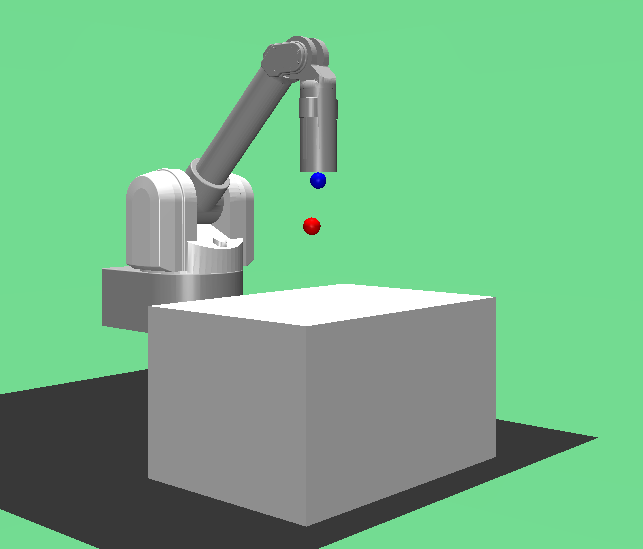
\includegraphics[width=0.4\linewidth]{4dof_setup.png} }}
    \qquad
    \subfloat[\centering 7 DOF]{{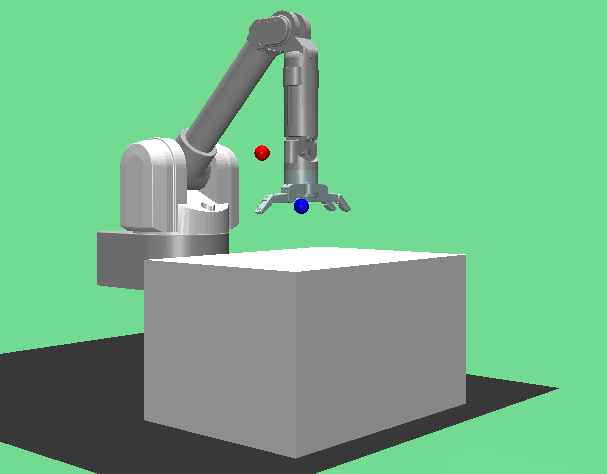
\includegraphics[width=0.4\linewidth]{7dof_setup.png} }}
    \caption{Reaching task experimental setup, blue: end effector, red: goal position}
    \label{figure_experimental_setup}
\end{figure}

\subsection{Uncalibrated Visual Servoing}

We present results for uncalibrated visual servoing in Table \ref{tab:results}. We find that uncalibrated visual servoing is
much more sample efficient than the reinforcement learning methods.

\begin{figure*}[thpb]
    \centering
    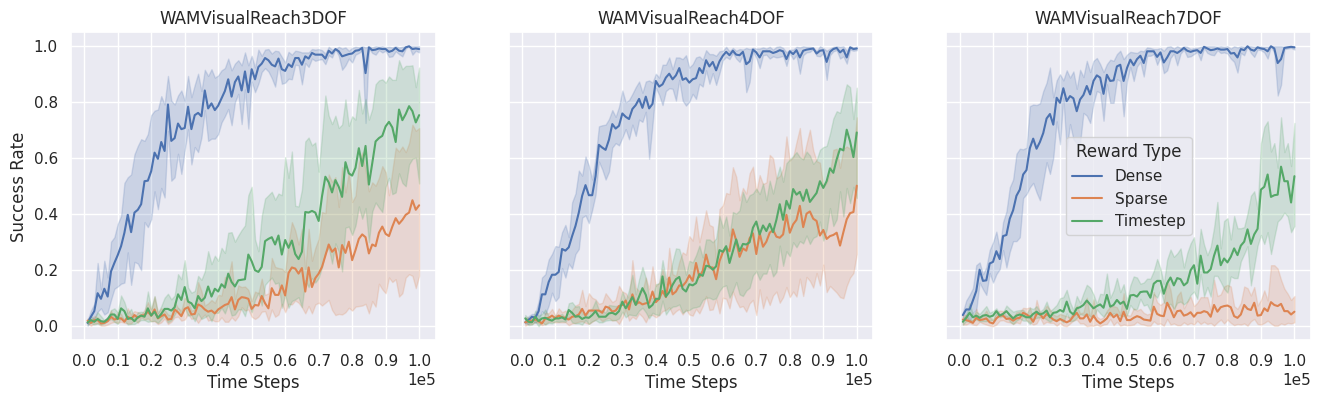
\includegraphics[width=\linewidth]{successes.reward_type.timesteps.png}
    \caption{Success rate of different reward functions on WAMVisualReach environment with 95\% confidence intervals}
    \label{fig:figure_reward_functions}
\end{figure*}

\subsection{Reinforcement Learning}

We first compare the effect of different reward function types and
different representations like neural networks and Neural Jacobians
on the sample efficiency and performance of reinforcement learning.


\subsubsection{Reward Type}

We compared the type of reward function used in reinforcement learning. As seen
in Fig. \ref{fig:figure_reward_functions}, we found that the dense reward
function was the most sample efficient, followed by the timestep reward
function, with the sparse reward function being the least sample efficient.
Notably, the 3 DOF results in Table \ref{tab:reward_type} show that the dense
reward function is at least two times as sample efficient in comparison to the
other reward functions. This demonstrates that reward shaping can significantly
improve sample efficiency.


\begin{table}[h] \caption{Reward Functions on WAMVisualReach 3DOF} \label{tab:reward_type}
    \begin{center}
        \begin{tabular}{|c|c|c|}
            \hline
            Reward Function & Success Rate & Sample Efficiency \\
            \hline
            Sparse & $0.07 \pm 0.08$ & $> 97000$  \\
            \hline
            Timestep & $0.16 \pm 0.13$ & $> 84500$  \\
            \hline
            Dense & $\textbf{0.93} \pm \textbf{0.13}$ & $\mathbf{41000} \pm \mathbf{11367}$ \\
            \hline
        \end{tabular}
    \end{center}
\end{table}

\begin{figure*}[thpb]
    \centering
    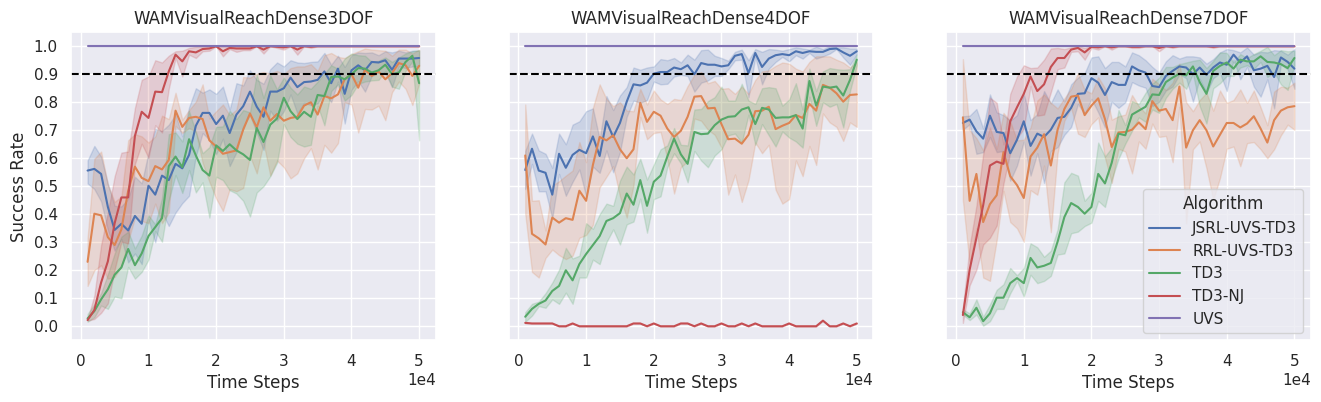
\includegraphics[width=\linewidth]{successes.alg.timesteps.png}
    \caption{Success rate on WAMVisualReach environment with different algorithms with 95\% confidence intervals}
    \label{figure_results}
\end{figure*}

\subsubsection{Neural Networks}

We evaluated the performance of neural network architectures with different
number of layers and neurons per layer.

Observing Fig. \ref{fig:arch}, we found that overall 2 layer neural networks
performed the best. We found that increasing the number of neurons per layer
improved sample efficiency with diminishing returns. In Fig. \ref{fig:arch}, we
note that 512 neurons per layer achieved a similar sample efficiency as 1024
neurons per layer. The remainder of experiments are conducted with 2 layer
neural networks with 512 neurons per layer.

We note that smaller neural network architectures, such as 1 layer of 128 neurons (18194 parameters) are capable of
achieving a final success rate of greater than 0.9, however, they are far less
sample efficient.

\subsubsection{Neural Jacobian}

We find that the Neural Jacobian works well for 3 and 7 DOF robot, improving
sample efficiency significantly. In fact, 12000 steps is approximately
equivalent to 1600 episodes of experience, which could be collected in less
than a day on a robot.

However, this technique does not work well for
the 4 DOF robot. We hypothesize that this is because during training the 4 DOF
robot has a tendency to move into singular configurations, which causes the
Neural Jacobian to become ill-conditioned, resulting in divergence during
training.

\subsection{Combined Approaches}
In this section, we compare methods that combine uncalibrated visual servoing
and reinforcement learning.

% \addtolength{\textheight}{-4cm}
% This command serves to balance the column
%                                   lengths % on the last page of the document
%                                   manually. It shortens % the textheight of
%                                   the last page by a suitable amount. % This
%                                   command does not take effect until the next
%                                   page % so it should come on the page before
%                                   the last. Make % sure that you do not
%                                   shorten the textheight too much.

\subsubsection{Residual Reinforcement learning}

We thought that RRL would be a promising technique for combining visual servoing
and reinforcement learning. However, we found that it did not work very well for
our task. While RRL was able to improve the performance in the initial steps
of training, it did not lead to a significant improvement in sample efficiency
when compared to TD3, and even performed worse in the 4 and 7 DOF cases.

\subsubsection{Jump Start Reinforcement Learning}

We find that JSRL works well for improving the sample efficiency of the robot. A
nice property of this technique is that during early training the policy still
has a reasonably high success rate, and can be considered more unlikely to fail
completely, which is important for training safely on a real robot. Another
advantage of JSRL in contrast to Residual Reinforcement Learning is that once
the target policy has been trained, it no longer has a dependency on the guide
policy, so it can be used independently. We find for the reaching task,
we can remove the guide policy after only 20000 steps of training.



\begin{table}[h] \caption{WAMVisualReach Results} \label{tab:results}
    \begin{center}
        \begin{tabular}{|c|c|c|c|c|}
            \hline
            Method & DOF & Success Rate & Reward & Sample Efficiency  \\
            \hline
            \multirow{3}{*}{UVS} & 3 & $1.00 \pm 0.00$ & $-1.38 \pm 0.05$  & $60 \pm 0$ \\ \cline{2-5}
                                 & 4 & $1.00 \pm 0.00$ & $-1.35 \pm 0.08$ & $80 \pm 0$ \\ \cline{2-5}
                                 & 7 & $1.00 \pm 0.00$ & $-1.16 \pm 0.08$ & $140 \pm 0$\\
            \hline
            \multirow{3}{*}{TD3} & 3 & $0.87 \pm 0.22$ & $-1.46 \pm 0.39 $ & $32400 \pm 7499$ \\ \cline{2-5}
                                 & 4 & $0.95 \pm 0.03$ & $-1.22 \pm 0.06$ & $39800 \pm 6431$ \\ \cline{2-5}
                                 & 7 & $0.96 \pm 0.03$ & $-1.14	\pm 0.11$ & $33200 \pm 2561$ \\
            \hline
            \multirow{3}{*}{TD3-NJ} & 3 & $1.00 \pm 0.00$ & $-1.18 \pm 0.09$ & $12200 \pm 1939$ \\ \cline{2-5}
                                 & 4 & $0.01 \pm 0.00$ & $-9.16 \pm 0.00$ & $-$ \\ \cline{2-5}
                                 & 7 & $1.00 \pm 0.00$ & $-1.04 \pm 0.07$ & $10400 \pm 3499$ \\
            \hline
            \multirow{3}{*}{RRL} & 3 & $0.93 \pm 0.08$ & $-1.35 \pm 0.20 $ & $> 50000$ \\ \cline{2-5}
                                 & 4 & $0.83 \pm 0.16$ & $-1.77 \pm 0.70 $ & $> 50000$ \\ \cline{2-5}
                                 & 7 & $0.79 \pm 0.11$ & $-2.05 \pm 0.80 $ & $> 50000$ \\
            \hline
            \multirow{3}{*}{JSRL} & 3 & $0.96 \pm 0.03$ & $-1.24 \pm 0.10$ & $30400 \pm 11741$ \\ \cline{2-5}
                                 & 4 & $0.98 \pm 0.01$ & $-1.12 \pm 0.06$ & $18800 \pm 2638$ \\ \cline{2-5}
                                 & 7 & $0.92 \pm 0.09$ & $-1.30 \pm 0.22$ & $21200 \pm 4956$ \\
            \hline
        \end{tabular}
    \end{center}
\end{table}

\subsection{Qualitative Evaluation}

Videos of the above experiments for qualitative evaluation are available at
\url{https://drive.google.com/drive/folders/1xF8Z_O7cWxLBhlskcR3WSw8cPf_iActh}.

We note that the reinforcement learning based methods generally have a smoother
and more direct trajectory compared to uncalibrated visual servoing. This
is reflective of the fact that reinforcement learning is capable of learning a
global visuomotor policy for the task.

The code for our experiments is available at
\url{https://github.com/steventango/visual-servoing}.

\section{CONCLUSION} \label{Conclusion}

We assessed the sample efficiency and performance of uncalibrated visual
servoing and reinforcement learning for a reaching task. We found that
techniques that combine visual servoing and reinforcement learning can greatly
improved the sample efficiency of reinforcement learning.

Future work includes comparing the performance of the different methods on a
real robot and comparing the different methods on a more challenging task such
as a pick and place task. Further research into improving the training stability
of the Neural Jacobian representation with reinforcement learning may also be
promising.

% \section*{APPENDIX}

% See Page \pageref{fig:arch} for Fig. \ref{fig:arch}.

\begin{figure*}[thpb]
    \centering
    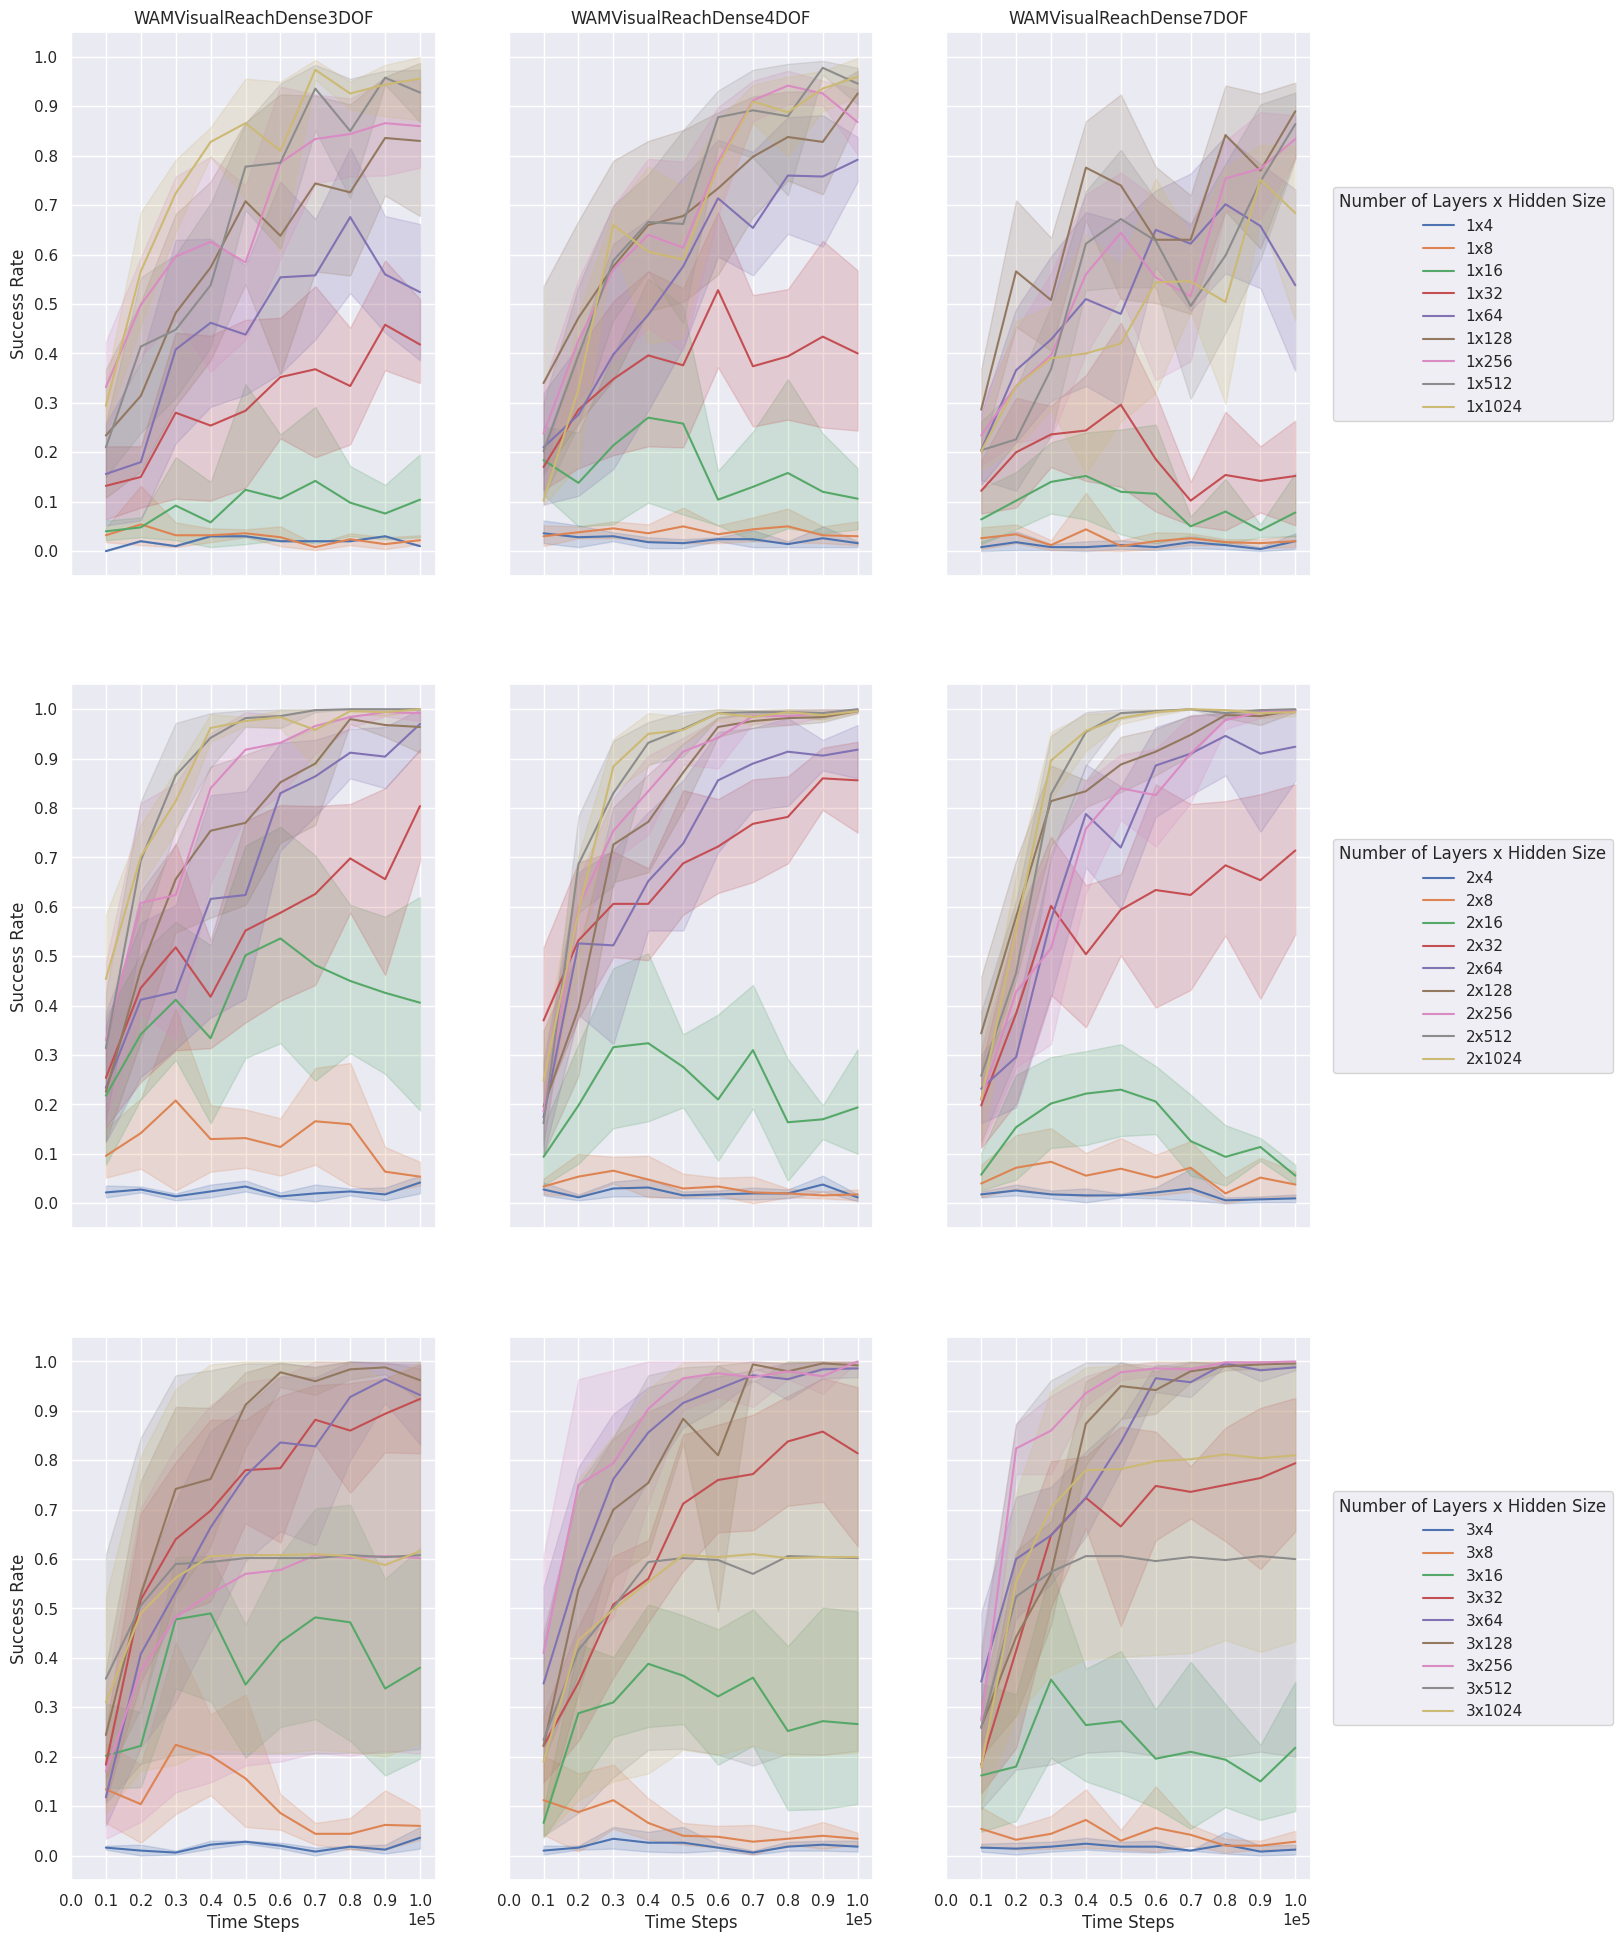
\includegraphics[width=\linewidth]{successes.arch.timesteps.png}
    \caption{Effect of neural network architecture on TD3}
    \label{fig:arch}
\end{figure*}

\section*{ACKNOWLEDGMENT}

We thank Dylan Miller for his advice on uncalibrated visual
servoing and reinforcement learning environment setup.

We acknowledge the support of the Natural Sciences and Engineering Research
Council of Canada (NSERC), [funding reference number 582453].

Cette recherche a été financée par le Conseil de recherches en sciences
naturelles et en génie du Canada (CRSNG), [numéro de référence 582453].

\bibliographystyle{IEEEtran}
\bibliography{IEEEabrv, bibliography}

\end{document}
